\documentclass[10pt]{article}

\usepackage{amsmath, amsthm, amssymb, amsfonts}
\usepackage{thmtools}
\usepackage{graphicx}
\usepackage{setspace}
\usepackage{geometry}
\usepackage{float}
\usepackage{hyperref}
\usepackage[utf8]{inputenc}
\usepackage[english]{babel}
\usepackage{framed}
\usepackage[dvipsnames]{xcolor}
\usepackage{tcolorbox}
\usepackage{mdframed}
\usepackage{tikz}
\usetikzlibrary{shapes, arrows, positioning}
\usepackage{enumerate}
\usepackage{listings}
\usepackage{fancyhdr}
\pagestyle{fancy}
\usepackage{graphicx}
\usepackage{booktabs}


\newcommand{\E}{\mathbb{E}}
\newcommand{\PP}{\mathbb{P}}

\newcommand{\independent}{\perp\mkern-9.5mu\perp}
\newcommand{\notindependent}{\centernot{\independent}}

\title{\textbf{An Evaluation of the Causal Effect of a Promotion Campaign on Software Usage}}
\author{Febriany Lete \\ Maysen Pagan}
\date{April 2024}

\begin{document}

\maketitle

\section{Introduction}
\section{Exploratory Data Analysis}

Before performing any causal analysis, we first explore the data for any missing values or outliers. There are no missing values in our data set, however, from a histogram of our response variable, we can see there exists one value that is negative. Since it is unknown if the revenue from this customer was input incorrectly and there is only one observation where the revenue is less than 0, we will remove this customer from our data set.

\begin{figure}[H]
  \centering
  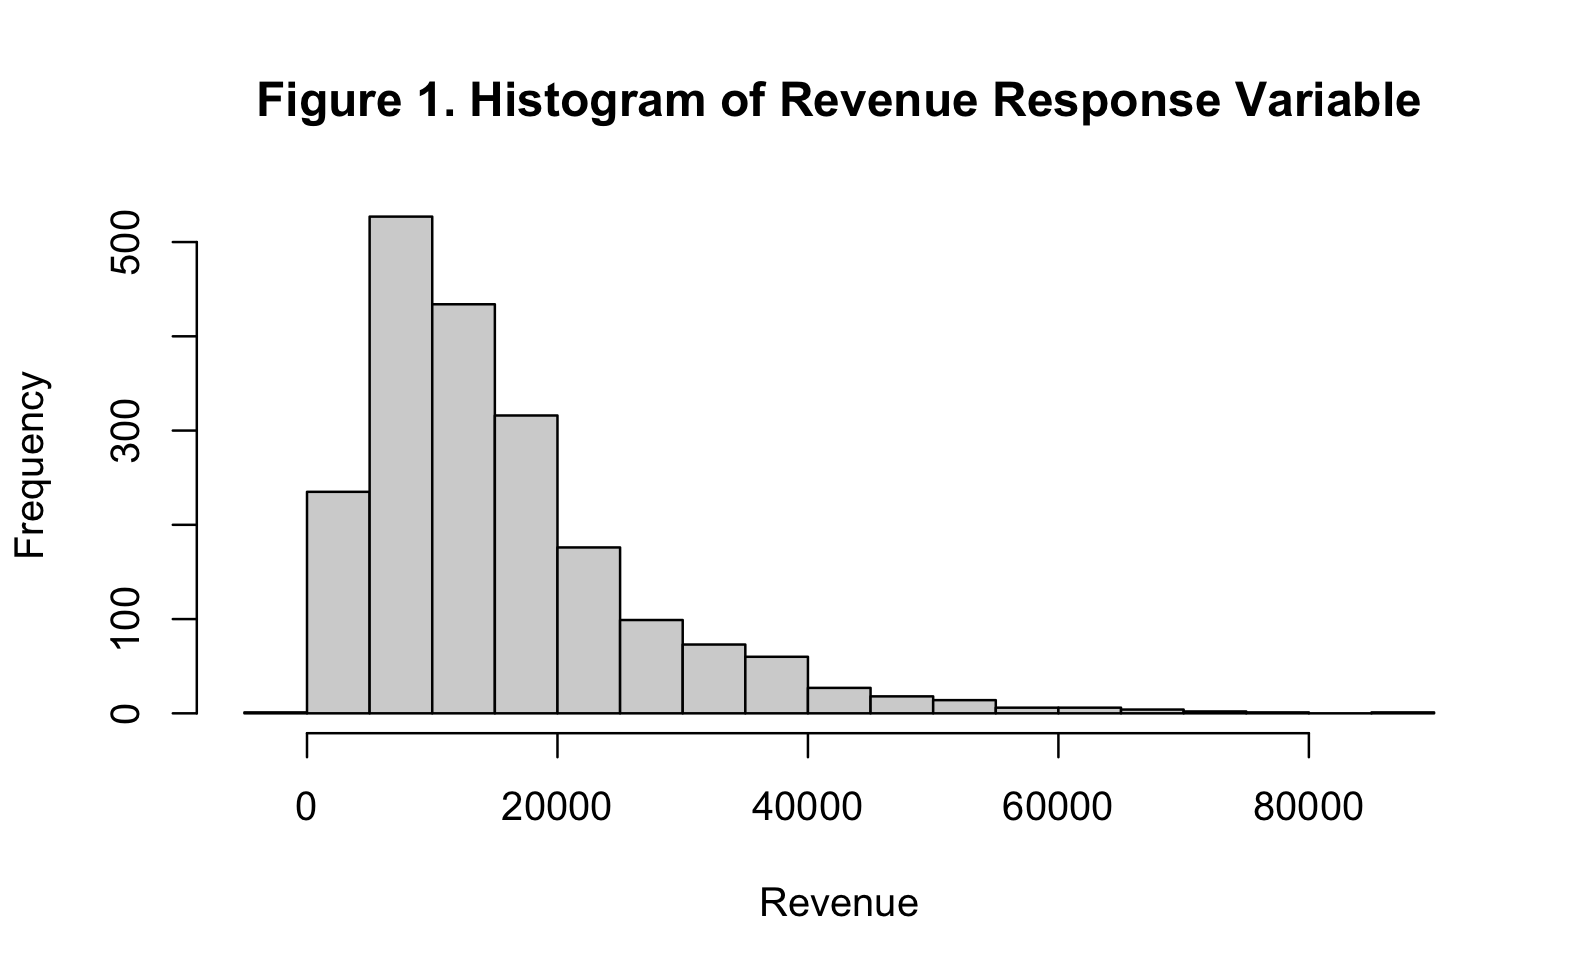
\includegraphics[width = 0.6\textwidth]{figs/response_hist.png}
\end{figure}

Next, we look at a correlation matrix of our quantitative variables. From Table 1, we can see a strong linear association of 0.95 between the number of PCs a customer has and the number of employees a customer has. Similarly, there is a large correlation of 0.88 between the size of the customer, given by their yearly total revenue, and the dollars spent on IT purchases by the customer. As a result, we choose to omit the dollars spend on IT purchases and the number of PCs the customer has from further analysis. \\

\begin{table}[ht]
\centering
\caption{Correlation Matrix of Reponse and Quantitative Predictors}\medskip
$
\begin{array}{l|ccccccccc}
                  & \text{IT Spend}    & \text{Employee Count}      & \text{PC Count}  & \text{Size}   & \text{Revenue}  \\ \hline
\text{IT Spend}          & 1.00        & 0.02                       & 0.02             & 0.88          & 0.74  \\
\text{Employee Count}    & 0.02        & 1.00                       & 0.95             & 0.02          & 0.23     \\
\text{PC Count}          & 0.02        & 0.95                       & 1.00             & 0.03          & 0.24     \\
\text{Size}              & 0.88        & 0.02                       & 0.03             & 1.00          & 0.86  \\
\text{Revenue}           & 0.74        & 0.23                       & 0.24             & 0.86          & 1.00     \\
\end{array}
$
\end{table}

\section{Methods and Analysis}
\subsection{Assumptions}

We then consider the three main identification assumptions to identify our average treatment effect: Positivity, Consistency, and Conditional Exchangeability.

\subsubsection{Positivity}

For the Positivity assumption, we observed the covariate balance plots for each of our covariates, comparing the distribution of the values between the treatment and control. These plots can be viewed in the Appendix. All plots show the pattern of an equal distribution of covariate values between those customers who received the discount and those who did not. For example, the first covariate balance plot for the employee count variable displays a skewed right distribution with the count ranging from 0 to about 500 employees both for customers who received a discount and customers who did not receive a discount. This demonstrates that for given values of each of the covariates, the probability of receiving the treatment and control are both non-zero. Therefore,
\[
0<p(A = a|X)<1,\:a\in\{0,1\}
\]
\subsubsection{Consistency}

We will also perform our causal analysis under the Consistency assumption which states that a customer's potential outcome under the observed treatment assignment is equal to the observed outcome for that customer. Therefore,
\[
\text{If} \; A_i = a, \text{then}\; Y_i = Y_i^{(a)}
\]
\subsubsection{Conditional Exchangeability}

For the Conditional Exchangeability assumption, we thought of possible variables that could be a confounder of the treatment-outcome relation. We believe that the size of the customer could be this confounder. The startup company might tend to give discounts to larger companies either to keep their loyalty or prevent them from purchasing from their competitors. In this sense, the size of the customer directly affects the treatment assignment. Additionally, the size of the customer may also directly affect the outcome because, for example, larger customers will most likely purchase more software than smaller customers and therefore bring in more revenue for the company. However, this size of the customer confounder can be observed in our data set through variables such as the number of employees the customer has or the binary variable that indicates if the customer has global offices. Larger businesses tend to have more employees as well as global offices. Since this confounder can be observed in our data set, we continue with the assumption of Conditional Exchangeability which states that
\[
\{Y^{(0)}, Y^{(1)}\} \independent{A|X}
\]
\subsection{Estimation}

Under the above assumptions, which are known as the three main identification assumptions, our parameter of interest, the average treatment effect (ATE), can be identified and then estimated using four methods.\\
\\
We first use the simplest estimator for the ATE which is the Outcome Regression (OR) Estimator. We also choose to estimate $\hat{\mu}$ for the OR function using linear regression with ordinary least squares estimator with $(1, A, X)$ as predictors. We then use non-parametric bootstrap to generate 1000 ATEs and estimated the standard error and confidence intervals for the OR estimator from these bootstrap estimates.
\[
\hat{\theta}_{ATE}^{or} = \E_n[\hat{\mu}(1,X) - \hat{\mu}(0,X)]
\]
Rather than modeling the outcome mechanism, we also model the treatment assignment mechanism using propensity score in the Inverse Probability Weighting (IPW) Estimator. This method is often used when partial information is available about the treatment assignment. In this campaign problem, we are uncertain of how the company chose to which customers they should provide discounts. Non-parametric bootstrap was also used to estimate standard error and obtain confidence intervals.
\[
\hat{\theta}_{ATE}^{ipw} = \E_n[\frac{A}{\hat{\mu}(X)}Y - \frac{1-A}{1-\hat{\mu}(X)}Y]
\]
The IPW approach, however, is not invariant to location transformation of the outcome and also is not stable leading to high variance. Therefore, we also calculate the ATE using the Hajek estimator which is invariant to location transformation of the outcome and is more stable (although this means it also has increased bias). Non-parametric bootstrap was used to estimate standard error and obtain confidence intervals.
\[
\hat{\theta}_{ATE}^{hajek} = \E_n\left[\frac{\frac{A}{\hat{\pi}(X)}}{\E_n[\frac{A}{\hat{\pi}(X)}]}Y - \frac{\frac{1-A}{1-\hat{\pi}(X)}}{\E_n[\frac{1-A}{1-\hat{\pi}(X)}]}Y\right]
\]
The OR function in the OR Estimator represents the outcome mechanism while the propensity score in the IPW and Hajek Estimators represents the treatment assignment mechanism. We also estimate the ATE using the Doubly Robust (DR) Estimator which combines both information and is unbiased if either the OR function or the propensity score is correctly specified. Similar to the previous estimators, non-parametric bootstrap was used to estimate standard error and obtain confidence intervals.
\[
\hat{\theta}_{ATE}^{hajek} = \E_n\left[\frac{A\{Y-\mu(1,X;\hat{\beta})\}}{\pi(X;\hat{\alpha})} + \mu(1,X;\hat{\beta}) - \frac{(1-A)\{Y-\mu(0,X;\hat{\beta})\}}{1-\pi(X;\hat{\alpha})} - \mu(0,X;\hat{\beta})\right]
\]
The propensity score was estimated using logistic regression with an order 1 polynomial. For each of the covariates, the estimated propensity scores were used to calculate $\frac{1}{n}\sum_{i=1}^{n}\{\frac{A_i}{\hat{\pi}(x_i)}-1\}\hspace{0.1cm}X_{i_{p}}$ for $p$ = 1,2,...,6 for 6 predictors. Bootstrap was used to calculate 1000 of these values for each covariate and 95\% confidence intervals were produced. The results are shown in Table 2 below. From this table, we can see that the value 0 falls in every confidence interval which suggests that my estimator of the propensity score satisfies the weighted balancing property for each of the covariates.

\begin{table}[htp]
\centering
\caption{Confidence Intervals for Covariate Balance Check}\medskip
\begin{tabular}{cccccc}
\toprule
Covariate             & Lower Bound            & Upper Bound   \\
\midrule
Global Flag           & -0.04                  & 0.05        \\
Major Flag            & -0.03                  & 0.06        \\
SMC Flag              & -0.06                  & 0.07        \\
Commercial Flag       & -0.07                  & 0.09        \\
Employee Count        & -6.77                  & 7.52        \\
Size                  & -8984.85               & 10340.57        \\
\bottomrule
\end{tabular}
\end{table}

Table 3 displays the ATE estimates, bootstrap standard errors, and bootstrap confidence intervals using the four methods above. 

\begin{table}[htp]
\centering
\caption{Estimated ATEs with Bootstrap Standard Errors and Confidence Intervals}\medskip
\begin{tabular}{cccccc}
\toprule
Method                & ATE                    & Standard Error        & Confidence Interval  \\
\midrule
Global Flag           & -0.04                  & 0.05                  &  \\
Major Flag            & -0.03                  & 0.06                  &  \\
SMC Flag              & -0.06                  & 0.07                  &  \\
Commercial Flag       & -0.07                  & 0.09                  &   \\
\bottomrule
\end{tabular}
\end{table}

From this table, we can see that all of the 95\% bootstrap confidence intervals do not contain zero suggesting that there is a positive causal effect between giving a customer a discount and the revenue received from that customer. We focus on the DR estimator because only one of the OR function or propensity score needs to be correctly specified for the estimator to be unbiased. We observe that the ATE is about 5,500 which means that on average, customers who received the discount would give the company \$5,500 more in revenue than those who did not receive the discount.

\subsection{Sensitivity Analysis}
We then performed sensitivity analysis to observe the extent to which the Conditional Exchangeability assumption might be violated. We chose our sensitivity parameters to range from $\frac{1}{2}$ to 2 and Figure 2 is a heatmap of the calculated effects with certain combinations of these parameters. We can see from the bottom right corner of the heatmap that the signs of our ATEs are sensitive only for larger sensitivity parameters. This suggests that when customers who receive a discount tend to bring in more revenue (which means the sensitivity parameters are larger than 1), then our results are sensitive. On the other hand, for customers who receive a discount and tend to bring in less revenue, our results are not sensitive and we can conclude that there is a positive causal effect.
\section{Conclusion}

\end{document}